\documentclass[12pt,a4paper]{article}
\topmargin=0pt
\headheight=0pt
\headsep=0pt
\textwidth=425pt

\usepackage{amssymb}
\usepackage{amsmath}
\usepackage{amstext}
\usepackage{amsthm}
\usepackage[dvips]{graphicx}

\begin{document}

\begin{titlepage}
\flushleft
\Huge Mixed Data-Type Circuit Modelling\\[40pt]
J. Rugis\\
\end{titlepage}

\LARGE
\pagebreak
\flushleft
\begin{table}
\LARGE
\begin{center}
\begin{tabular}{|c|l|l|l|l|}
\hline Operator & Operation & \multicolumn{2}{l|}{Arguments} & Result \\
\hline + & addition & numeric & numeric & numeric\\
\hline - & subtraction & numeric & numeric & numeric\\
\hline - & negation & numeric & none & numeric\\
\hline (blank) & multiplication &  numeric & numeric & numeric\\
\hline  / & division &  numeric & numeric & numeric\\
\hline  $<$ & less than &  numeric & numeric & boolean\\
\hline  $>$ & greater than &  numeric & numeric & boolean\\
\hline  $=$ & equal to &  numeric & numeric & boolean\\
\hline  $\wedge$ & and &  boolean & boolean & boolean\\
\hline  $\vee$ & or &  boolean & boolean & boolean\\
\hline  $\oplus $ & exclusive or &  boolean & boolean & boolean\\
\hline $\Rightarrow$ & implication & boolean & boolean & boolean\\
\hline
\end{tabular}
\end{center}
\end{table}
Operator Summary

\pagebreak
\flushleft
\emph{When required, convert the Boolean ``true" to the real number 1 and the Boolean ``false" to the real number 0.}

\pagebreak
\flushleft
A boolean expression:
\begin{equation*}
i=v/R \text{, where }(i,v,R) \in \mathbb R
\end{equation*}\\[80pt]
\pagebreak
\flushleft
A boolean expression:
\begin{equation*}
i=v/R \text{, where }(i,v,R) \in \mathbb R
\end{equation*}\\[80pt]
Ohm's Law:
\begin{equation*}
\vDash (i=v/R)
\end{equation*}

\pagebreak
\flushleft
\begin{figure}[ht]
\centering
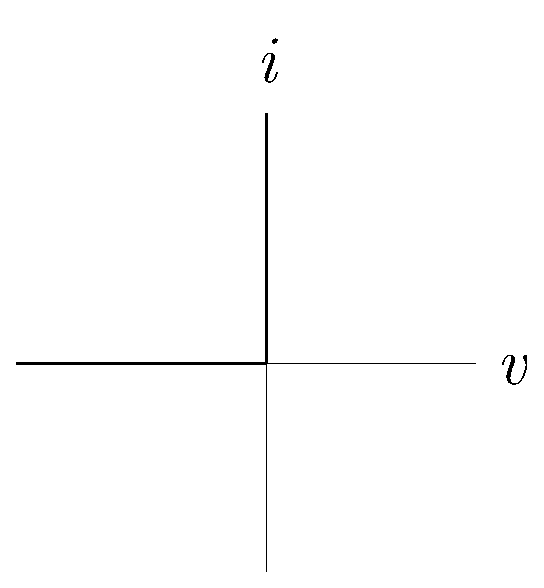
\includegraphics{d1large}
\end{figure}
Diode characteristic $vi$ curve.

\pagebreak
\flushleft
\begin{enumerate}
\item Either the voltage or the current is zero,
\item if the current is zero then the voltage is less than or equal to zero,
\item and if the voltage is zero then the current is greater than or equal to zero.
\end{enumerate}

\pagebreak
\flushleft
\begin{gather*}
(v=0) \vee (i=0) \\
(i=0) \Rightarrow (v \le 0) \\
(v=0) \Rightarrow (i \ge 0)
\end{gather*}\\[30pt]
\pagebreak
\flushleft
\begin{gather*}
(v=0) \vee (i=0) \\
(i=0) \Rightarrow (v \le 0) \\
(v=0) \Rightarrow (i \ge 0)
\end{gather*}\\[30pt]
\begin{multline*}\vDash \Big(
\big((v=0) \vee (i=0)\big) \wedge \\
\big((i=0) \Rightarrow (v \le 0)\big) \wedge \\
\big((v=0) \Rightarrow (i \ge 0)\big) \Big)
\end{multline*}

\pagebreak
\flushleft
\begin{equation*}
\begin{bmatrix}
\mathbf{0} &\mathbf{0} &\mathbf{A}\\
-\mathbf{A}^T &\mathbf{1} &\mathbf{0}\\
\mathbf{0} &\mathbf{M} &\mathbf{N}
\end{bmatrix}
\begin{bmatrix}
\mathbf{e}\\
\mathbf{v}\\
\mathbf{i}
\end{bmatrix}
=
\begin{bmatrix}
\mathbf{0}\\
\mathbf{0}\\
\mathbf{u}_s
\end{bmatrix}\label{eq:st}
\end{equation*}\\[40pt]
\pagebreak
\flushleft
\begin{equation*}
\begin{bmatrix}
\mathbf{0} &\mathbf{0} &\mathbf{A}\\
-\mathbf{A}^T &\mathbf{1} &\mathbf{0}\\
\mathbf{0} &\mathbf{M} &\mathbf{N}
\end{bmatrix}
\begin{bmatrix}
\mathbf{e}\\
\mathbf{v}\\
\mathbf{i}
\end{bmatrix}
=
\begin{bmatrix}
\mathbf{0}\\
\mathbf{0}\\
\mathbf{u}_s
\end{bmatrix}\label{eq:st}
\end{equation*}\\[40pt]
\begin{equation*}
\begin{bmatrix}
\mathbf{M} &\mathbf{N}
\end{bmatrix}
\begin{bmatrix}
\mathbf{v} \\ \mathbf{i}
\end{bmatrix}
=\mathbf{u}_s
\end{equation*}\\[20pt]
\pagebreak
\flushleft
\begin{equation*}
\begin{bmatrix}
\mathbf{0} &\mathbf{0} &\mathbf{A}\\
-\mathbf{A}^T &\mathbf{1} &\mathbf{0}\\
\mathbf{0} &\mathbf{M} &\mathbf{N}
\end{bmatrix}
\begin{bmatrix}
\mathbf{e}\\
\mathbf{v}\\
\mathbf{i}
\end{bmatrix}
=
\begin{bmatrix}
\mathbf{0}\\
\mathbf{0}\\
\mathbf{u}_s
\end{bmatrix}\label{eq:st}
\end{equation*}\\[40pt]
\begin{equation*}
\begin{bmatrix}
\mathbf{M} &\mathbf{N}
\end{bmatrix}
\begin{bmatrix}
\mathbf{v} \\ \mathbf{i}
\end{bmatrix}
=\mathbf{u}_s
\end{equation*}\\[20pt]
\begin{equation*}
\begin{bmatrix}
a &b
\end{bmatrix}
\begin{bmatrix}
v_b \\ i_b
\end{bmatrix}
=u_b
\end{equation*}\\[20pt]

\pagebreak
\flushleft
Selectors:
\begin{gather*}
rx + sy = c\\
\text{where }  (r,s) \in \mathbb B , \: (x,y,c) \in \mathbb R \\
\text{and } \vDash (r \oplus s)
\end{gather*}

\pagebreak
\flushleft
\begin{gather*}
rv + si=0 \label{eq:d1}\\
r \oplus s \label{eq:d2}\\
(i=0) \Rightarrow (v \le 0) \label{eq:d3}\\
(v=0) \Rightarrow (i \ge 0) \label{eq:d4}
\end{gather*}\\[40pt]
\pagebreak
\flushleft
\begin{gather*}
rv + si=0 \label{eq:d1}\\
r \oplus s \label{eq:d2}\\
(i=0) \Rightarrow (v \le 0) \label{eq:d3}\\
(v=0) \Rightarrow (i \ge 0) \label{eq:d4}
\end{gather*}\\[40pt]
\begin{gather*}
\begin{bmatrix} r & s \end{bmatrix}
\begin{bmatrix} v \\ i \end{bmatrix}=0 \label{eq:dsel1} \\
\text{where }\begin{bmatrix} r & s \end{bmatrix} 
\in \left\{ \begin{bmatrix} 0 & 1 \end{bmatrix},
\begin{bmatrix} 1 & 0 \end{bmatrix} \right\} \label{eq:dsel2}
\end{gather*}

\pagebreak
\flushleft
\begin{figure}[ht]
\centering
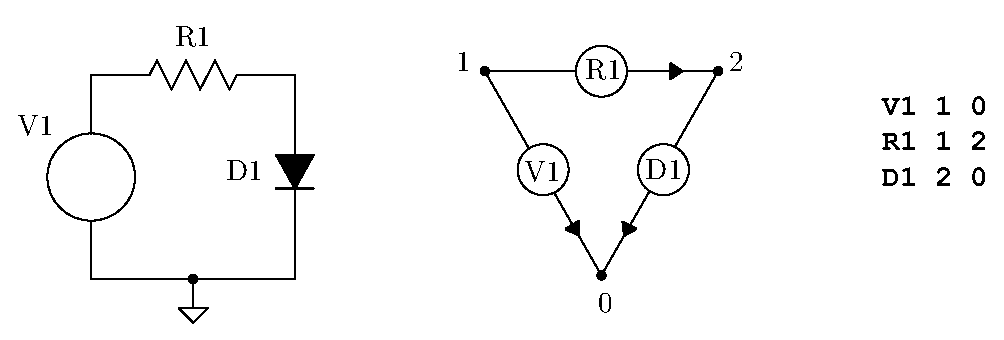
\includegraphics{c1large}
\end{figure}
A simple circuit.

\pagebreak
\flushleft
\begin{gather*}
\left[\begin{array}{cccccccc|c}
0 &0 &0 &0 &0 &1 &1 &0 &0\\
0 &0 &0 &0 &0 &0 &-1 &1 &0\\
-1 &0 &1 &0 &0 &0 &0 &0 &0\\
-1 &1 &0 &1 &0 &0 &0 &0 &0\\
0 &-1 &0 &0 &1 &0 &0 &0 &0\\
0 &0 &1 &0 &0 &0 &0 &0 &V_{V1}\\
0 &0 &0 &1 &0 &0 &-R_{R1} &0 &0\\
0 &0 &0 &0 &r_{D1} &0 &0 &s_{D1} &0
\end{array}\right]
\label{eq:ag1}
\end{gather*}\\

\pagebreak
\flushleft
\begin{gather*}
\det \mathbf T = s_{D1}-r_{D1}R_{R1}
\end{gather*}\\[20pt]
\pagebreak
\flushleft
\begin{gather*}
\det \mathbf T = s_{D1}-r_{D1}R_{R1}
\end{gather*}\\[20pt]
\begin{gather*}
\begin{array}{l|c}
\left[ \; r_{D1} \; \; s_{D1} \; \right] &\det \mathbf T \\ \hline
\left[ \; 0 \; \; 1 \; \right] &1 \\
\left[ \; 1 \; \; 0 \; \right] &-R_{R1}
\end{array}
\end{gather*}\\[20pt]
\pagebreak
\flushleft
\begin{gather*}
\det \mathbf T = s_{D1}-r_{D1}R_{R1}
\end{gather*}\\[20pt]
\begin{gather*}
\begin{array}{l|c}
\left[ \; r_{D1} \; \; s_{D1} \; \right] &\det \mathbf T \\ \hline
\left[ \; 0 \; \; 1 \; \right] &1 \\
\left[ \; 1 \; \; 0 \; \right] &-R_{R1}
\end{array}
\end{gather*}\\[20pt]
\begin{gather*}
\begin{array}{l|c|l}
\left[ \; r_{D1} \; \; s_{D1} \; \right] &\det \mathbf T &\text{constraints} \\ \hline
\left[ \; 0 \; \; 1 \; \right] &1 &\text{none} \\
\left[ \; 1 \; \; 0 \; \right] &-R_{R1} &R_{R1} > 0 
\end{array}
\end{gather*}\\

\pagebreak
\flushleft
\begin{gather*}
v_{D1}=\frac{s_{D1}V_{V1}}{\det \mathbf T} \\ \\
i_{D1}=\frac{-r_{D1}V_{V1}}{\det \mathbf T} \\
\end{gather*}
\pagebreak
\flushleft
\begin{gather*}
v_{D1}=\frac{s_{D1}V_{V1}}{\det \mathbf T} \\ \\
i_{D1}=\frac{-r_{D1}V_{V1}}{\det \mathbf T} \\
\end{gather*}
\begin{gather*}
\begin{array}{l|c|c|c}
\left[ \; r_{D1} \; \; s_{D1} \; \right] &\text{constraints} &v_{D1} &i_{D1} \\ \hline
\left[ \; 0 \; \; 1 \; \right] &\text{none} &V_{V1} &0 \\
\left[ \; 1 \; \; 0 \; \right] &R_{R1} > 0 &0 &V_{V1}/R_{R1} 
\end{array}
\end{gather*}\\

\pagebreak
\flushleft
\begin{gather*}
\begin{array}{c|c|c}
\text{constraints} &v_{D1} &i_{D1} \\ \hline
v_{D1} \le 0 &V_{V1} &0 \\
i_{D1} \ge 0, R_{R1} > 0 &0 &V_{V1}/R_{R1} 
\end{array}
\end{gather*}\\[30pt]
\pagebreak
\flushleft
\begin{gather*}
\begin{array}{c|c|c}
\text{constraints} &v_{D1} &i_{D1} \\ \hline
v_{D1} \le 0 &V_{V1} &0 \\
i_{D1} \ge 0, R_{R1} > 0 &0 &V_{V1}/R_{R1} 
\end{array}
\end{gather*}\\[30pt]
\begin{gather*}
\begin{array}{c|c|c}
\text{constraints} &v_{D1} &i_{D1} \\ \hline
V_{V1} \le 0 &V_{V1} &0 \\
V_{V1} \ge 0, R_{R1} > 0 &0 &V_{V1}/R_{R1} 
\end{array}
\end{gather*}\\

\pagebreak
\flushleft
\begin{multline*}\vDash \Big(
\big((V_{V1} \!\le \! 0)  \!\implies \! (v_{D1} \!= \!V_{V1})  \!\wedge \! (i_{D1} \!= \!0)\big)  \!\wedge \! \\
\big((V_{V1}  \!>\! 0)  \!\wedge \! (R_{R1} > 0)  \!\implies \! (v_{D1} \!= \!0)  \!\wedge \! (i_{D1} \!= \!V_{V1}/R_{R1})\big)
\Big)\end{multline*}

\pagebreak
\flushleft
\begin{figure}[ht]
\centering
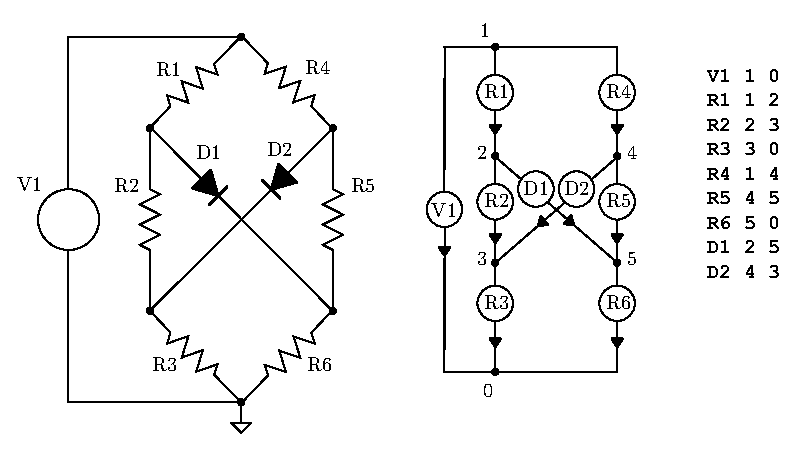
\includegraphics{c4large}
\end{figure}
A more complex example.

\end{document}